\documentclass{book}
\usepackage{graphicx}
\usepackage[english]{babel}
\usepackage{amsthm}
\usepackage{amssymb}
\usepackage{amsfonts}
\usepackage{mdframed}
\usepackage{physics}
\usepackage{tikz}
\usepackage[a4paper, margin=1in]{geometry}
\geometry{a4paper, margin=1in}
\usepackage{xcolor}
\usetikzlibrary{arrows.meta}
\usetikzlibrary{angles,quotes}
\graphicspath{ {./images/} }
\usepackage{svg}
\usepackage{subcaption}
\usepackage{bm}
\usepackage{empheq}
\usepackage{cancel}
\usetikzlibrary{decorations.text}
\usepackage[most]{tcolorbox}
\usepackage{tensor}
%3D
\usepackage{mathtools}
\usepackage{booktabs}
\usepackage{array}
\newcolumntype{C}{>{$}c<{$}}
\usepackage{tikz-3dplot}
\usepackage{appendix}
\usepackage{pgfplots}
\usetikzlibrary{shapes.geometric}
\usetikzlibrary{calc,patterns,angles,quotes}
%Tikz Library
\usetikzlibrary{angles, quotes, intersections}
\usepackage[bb=dsserif]{mathalpha}
\usetikzlibrary{decorations.pathmorphing}

\tikzset{snake it/.style={decorate, decoration=snake}}

\usepackage{etoolbox} % ifthen
\usepackage[outline]{contour} % glow around text
\usetikzlibrary{calc} % for adding up coordinates
\usetikzlibrary{decorations.markings,decorations.pathmorphing}
\usetikzlibrary{angles,quotes} % for pic (angle labels)
\usetikzlibrary{arrows.meta} % for arrow size
\usepackage{xfp} % higher precision (16 digits?)

\usepackage{tcolorbox}

\def\innerproduct#1#2{{\langle #1},{#2 \rangle}}
\renewcommand{\braket}[2]{\langle#1|#2\rangle}

%https://osl.ugr.es/CTAN/macros/latex/contrib/tcolorbox/tcolorbox.pdf
\tcbuselibrary{breakable}
\tcbset{%any default parameters
	width=0.7\textwidth,
	halign=justify,
	center,
	breakable,
	colback=white    
}

\newenvironment{aside}
{\begin{mdframed}[style=0,%
		leftline=false,rightline=false,leftmargin=2em,rightmargin=2em,%
		innerleftmargin=0pt,innerrightmargin=0pt,linewidth=0.75pt,%
		skipabove=7pt,skipbelow=7pt]\small}
	{\end{mdframed}}

\renewcommand{\cleardoublepage}{\clearpage}

\title{Complex Variables and Vector Spaces}
\author{Dominik Szablonski}
\newtheorem{law}{Law}
\newtheorem{klaw}{Law}

\newtcbtheorem{Definitions}{Definition}%
{colback=blue!5!white,colframe=blue!75!black,width=\textwidth,fonttitle=\bfseries}{}

\newtcbtheorem{Theorems}{Theorem}%
{colback=red!5!white,colframe=red!75!black,width=\textwidth,fonttitle=\bfseries}{}

\newtcbtheorem{Examples}{Example}%
{colback=yellow!5!white,colframe=yellow!75!black,width=\textwidth,fonttitle=\bfseries}{}
\def\doubleunderline#1{\underline{\underline{#1}}}

\newtheorem*{theorem}{Theorem}


\setlength\parindent{0pt}
\pgfplotsset{compat=1.18}
\begin{document}
\maketitle

\tableofcontents

\chapter{Vector Spaces}
We wish to generalise the idea of a vector and field. Let us first define a field,
\begin{Definitions}{Fields}{}
	A field $\mathbb{F}$ is a set with 2 binary operations defined on it, addition $(+)$ and multiplication $(\cdot)$. The following axioms hold $\forall a,b,c \in \mathbb{F}$,
	\begin{enumerate}
		\item \textit{Associativity}, \begin{align}
			a + (b + c) = (a + b) + c &&
			a \cdot (b\cdot c) = (a\cdot b) \cdot c
		\end{align}
		\item \textit{Commutativity}, \begin{align}
			a + b = b + a &&
			a\cdot b = b\cdot a
		\end{align}
		\item \textit{Identity}. $\exists 0, 1 \in \mathbb{F}$ such that,
		\begin{align}
			a + 0 = a &&
			a\cdot 1 = a
		\end{align}
		\item \textit{Additive inverse.} $\forall a \in \mathbb{F}, \exists -a \in \mathbb{F}$ such that,
		\begin{equation}
			a + (-a) = 0.
		\end{equation}
		\item \textit{Multiplicative inverse.} $\forall a \in \mathbb{F}, \exists a^{-1} \in \mathbb{F}$ such that,
		\begin{equation}
			a \cdot a^{-1} = 1.
		\end{equation}
	\end{enumerate}
\end{Definitions}
We can then define a vector space,
\begin{Definitions}{Vector Space}{}
	Let $\mathbb{F}$ be a field. A vector space $V$ over $\mathbb{F}$ is a set of objects $\vb{u}, \vb{v}, \vb{w},\ldots$ which satisfy,
	\begin{enumerate}
		\item \textit{Addition.} The set is closed under addition, such that $\vb{u}, \vb{v} \in V \implies \vb{w} = \vb{u} + \vb{v} \in V$. This operation is commutative and associative.
		\item \textit{Scalar multiplication.} The set is closed under multiplication by a scalar, i.e., $\vb{u} \in V \implies \lambda \vb{u}\in V$ for $\lambda \in \mathbb{F}$. Scalar multiplication is associative and distributive.
		\item \textit{Null vector.} $\exists \vb{0}, \vb{u} + \vb{0} = \vb{u}$.
		\item \textit{Negative vector.} $\forall \vb{u} \in V, \exists -\vb{u} \in V$ such that,
		\begin{equation}
			\vb{u} + (-\vb{u}) = 0.
		\end{equation} 
	\end{enumerate}
\end{Definitions}
\section{Linear Independence}
If vectors are linearly independent, then they cannot be written as a combination of each other. Let us write down the formal definition,
\begin{Definitions}{Linear Independence}{}
	A set of vectors $\left\{\vb{u}_i \text{ for } i = 1, 2, \ldots, n\right\}$ is linearly independent if the equation,
	\begin{equation}
		\sum_j^n \lambda_j\vb{u}_j = \vb{0}
	\end{equation}
	has only 1 solution, $\forall i : \lambda_i = 0$.
\end{Definitions}
\section{Postulate of Dimensionality and Basis Vectors}
\begin{Definitions}{Dimensionality}{}
	A vector space $V$ has dimensions $N$ if it can accommodate no more than $N$ linearly independent vectors $\vb{u}_j$.
\end{Definitions}
We often denote $N$ dimensional vector spaces over a field $\mathbb{F}$ as $\mathbb{F}^N$, or more generally $V_N$. We are often also interested in the \textit{span} of a vector space.
\begin{Definitions}{Span}{}
	The span of a set of vectors $\left\{\vb{u}_i, for i=1,2,\ldots,n\right\}$ is the set of all vectors which can be written as a linear combination of $\vb{u}_i$.
\end{Definitions}
The above definition naturally leads to the below theorem,
\begin{Theorems}{}{}
	In an $N$-dimensional vector space $V_N$, any vector $\vb{u}$ can be written as a linear combination of $N$ linearly independent basis vectors $\vb{e}_j$.
\end{Theorems}
\begin{proof}
	Since there are no more than $N$ linearly independent vectors, the set of vectors $\left\{\vb{e}_i\right\}_{i=1}^{N} + \vb{u}$ must be linearly dependent. Therefore, there must be a relation of the form,
	\begin{equation}
		\sum_{i=1}^{N} \lambda_i\vb{e}_i + \lambda_0\vb{u} = \vb{0},
	\end{equation}
	where $\vb{u} \in V_N$ is an arbitrary vector and $\exists \lambda_i \neq 0$. From the definition of linear dependence, we require $\lambda_0 \vb{u}_0 \neq 0$, so,
	\begin{equation}
		\vb{u} = - \frac{1}{\lambda_0}\sum_{i=1}^{N}\lambda_i\vb{e}_i = \sum_i^Nu_i\vb{e}_i
	\end{equation}
	where $u_i = -\frac{\lambda_i}{\lambda_0}$.
\end{proof}
From the above theorem, we are able to define the \textbf{basis} of a vector space,
\begin{Definitions}{Basis}{}
	Any set of $N$ linearly independent vectors in $V_n$ is called a \textbf{basis}, and then \textbf{span} $V_N$, or synonymously, they are \textbf{complete} if $N$ is finite.
\end{Definitions}
This allows us to write any vector $\vb{v} \in V_N$ as,
\begin{equation}
	\vb{v} = \sum_i^Nv_i\vb{e}_i
\end{equation}
where $\vb{e}_i$ is any complete basis.
\section{Linear Subspaces}
We can consider a subspace of $V_N$ as a vector space spanned by a set of $M < N$ linearly independent vectors. The subspace $V_M$ must satisfy the following properties,
\begin{enumerate}
	\item It must contain the zero vector $\vb{0}$.
	\item It must be closed under addition and scalar multiplication.
\end{enumerate}
An example of a subspace would be the subspace of $\mathbb{R}^3$ which is the set of vectors $(x,y,0)$, where $x,y \in \mathbb{R}$ which define the $xy$-plane in $\mathbb{R}^3$. This is a case of a more general result,
\begin{Theorems}{Subspaces}{}
	Any set of $M$ $(M \leq N)$ linearly independent vectors $\left\{\vb{e}_i\right\}^M_{i=1}$ in $V_N$ span a subspace $V_M$ of $V_N$.
\end{Theorems}
However, counterexamples do exist such as the set of vectors lying within a unit circle $\left\{(x,y):x^2+y^2 \leq 1\right\}$ which cannot be a subspace of $\mathbb{R}^3$ This is because we can choose a $\lambda$ such that $\lambda x_1$ or $\lambda y_1 > 1$ lies outside of the unit circle, and thus is not closed under multiplication.
\section{Normed Spaces}
We wish to now generalise length in order to define the closeness of vectors. We do this by defining a \textit{norm}.
\begin{Definitions}{Norm}{}
	Give a vector space $V$ over a field $\mathbb{F}$, a norm on $V$ is a real-valued function $p : V \to \mathbb{R}$ with the following properties,
	\begin{enumerate}
		\item \textbf{Triangle Inequality}, $p(\mathbf{x} + \mathbf{y}) \leq p(\mathbf{x}) + p(\mathbf{y}), \forall \mathbf{x}, \mathbf{y} \in V$
		\item \textbf{Absolute Homogeneity}, $p(sx) = \abs{s}p(\vb{x}), \forall \mathbf{x} \in V, \forall s \in \mathbb{R}$.
		\item \textbf{Positive Definiteness}, $\forall \vb{x} \in V, p(x) \geq 0; p(x) = 0 \iff x = 0$.
	\end{enumerate}
\end{Definitions}
For a vector space $V_N$ and two vectors $\vb{u},\vb{v} \in V_N$, the distance between them is given by $\norm{\vb{u} - \vb{v}}$. There are different types of norms, some of which are defined in sections below. 
\subsection{Supremum Norm}
$\forall \vb{x} \in V_N$ where $x_i$ are the components in a given basis, the we define the \textit{supremum} or \textit{infinity} norm.
\begin{Definitions}{Supremum Norm}{}
	\begin{equation}
		\norm{\vb{x}}_S = \norm{\vb{x}}_{\infty} = \max_i\abs{x_i}.
	\end{equation}
\end{Definitions}
It can be shown that, since $\abs{a + b} \leq \abs{a} + \abs{b}$ $\forall a,b \in \mathbb{R}$ or $\forall a,b \in \mathbb{C}$,
\begin{equation}
	\begin{split}
		\norm{\vb{x} + {y}} = \max_i\abs{x_i + y_i} & \leq \max_i\left(\abs{x_i} + \abs{y_i}\right) \\
		& \leq \max_i\abs{x_i} + \max_j\abs{y}
	\end{split}
\end{equation}
\subsection{1-Norm}
$\forall \vb{x} \in V_N$ where $x_i$ are the components of $\vb{x}$, we define the 1-norm,
\begin{Definitions}{1-Norm}{}
	\begin{equation}
		\norm{x}_1 = \sum_{i=1}^N \abs{x_i}.
	\end{equation}
\end{Definitions}
\section{Completeness}
\subsection{Cauchy Sequences}
\begin{Definitions}{Cauchy Sequence}{}
	A sequence $\left\{a_n\right\}_{n=0}^{\infty}$, $a_n \in V$ and $V$ is a normed vector space is Cauchy if $\forall \epsilon > 0, \exists N > 0$ such that $\forall n,m > N, \norm{a_n - a_m} < \epsilon$.
\end{Definitions}{}{}
Let us consider some sequences and show if they are Cauchy.
\subsubsection{Sequences over $\mathbb{R}$}
	\begin{figure}
		\centering
	\begin{tikzpicture}
		\begin{axis}[%
			,axis x line = bottom,axis y line = left
			,ytick=\empty, xtick=\empty
			,ymax=5, xmax=3 % or enlarge y limits=upper
			]
			\addplot+[const plot, no marks, very thick, color=black] coordinates {(0,4) (0.5,1) (1,0.444) (1.5,0.25) (2,0.16) (2.5,0.111)};
			\addplot+[no marks, thick, dashed, color=red, domain=0:5,samples=100] plot {1/(\x*\x) };
			\node[anchor = west] at (0.5,4) {$\displaystyle\frac{1}{(m+1)^2}$};
			\node[anchor = south] at (2.5,0.111) {$\displaystyle\frac{1}{n^2}$};
			\node at (0.8, 2.5) {$\displaystyle\frac{1}{x^2}$};
		\end{axis}
	\end{tikzpicture}
	\caption{Graphical proof used in example 1.}
	\label{fig:proof1}
\end{figure}
\begin{Examples}{$a_n = \sum_{i=1} \frac{1}{i^2}$}{}
	A sequence in $\mathbb{R}$ with $\norm{a} = \abs{a}$ is
	\begin{equation}
		a_n =  \sum_{i=1}^{n}\frac{1}{i^2}.
	\end{equation}
	Is this sequence Cauchy?
\end{Examples}
	For $n > m$, let us write,
	\begin{equation}
		\abs{a_n - a_m} = \sum_{i=m=1}^{n} \frac{1}{i^2}
	\end{equation}
	If we consider the sum as the integral over a series of step functions, then we can consider an approximation of this integral as $\frac{1}{x^2}$, as in figure \ref{fig:proof1}. Thus,
	\begin{equation}
		\begin{split}
			\sum_{i = m+1}^{n}\frac{1}{i^2} & \leq \int_m^n \frac{1}{x^2}\dd{x} \\
			& = \frac{1}{n} - \frac{1}{m} \leq \frac{1}{n} \leq \frac{1}{N}.
		\end{split}
	\end{equation}
	Let us now choose $N > \frac{1}{\epsilon}$, so that we find,
	\begin{equation}
		\abs{a_n - a_m} < \epsilon
	\end{equation}
	thus the sequence is Cauchy. $\qed$
\begin{Examples}{$a_n = n$}
	Consider a sequence $a_n = n$. Is this sequence Cauchy?
\end{Examples}
Let us choose $\epsilon = 1$, $n = N+1$, and $m = N + 3$
	\begin{equation}
		\abs{a_n - a_m} = 2 > \epsilon
	\end{equation}
	so the sequence is not Cauchy. $\qed$
\subsubsection{Cauchy sequences of functions}
We can also apply similar proofs to functions.
\begin{Examples}{$f:\left[0,1\right]\to \mathbb{R}$, $f_n(x) = \frac{x}{n}$.}{}
	Consider $f:\left[0,1\right]\to \mathbb{R}$ where $f_n(x) = \frac{x}{n}$. Is this function Cauchy?
\end{Examples}
Let $n > m$,
	\begin{equation}
		\begin{split}
		\norm{f_n - f_m}_1 & = \int_0^1 \abs{\frac{x}{n} - \frac{x}{m}}\dd{x} \\
		& = \abs{\frac{1}{n} - \frac{1}{m}}\int_0^1x \dd{x} \\
		& = \frac{1}{2}\abs{\frac{1}{n} - \frac{1}{m}}\leq \frac{1}{2}\left(\abs{\frac{1}{n}} + \abs{\frac{1}{m}}\right) \leq \frac{1}{2}\frac{2}{N} = \frac{1}{N}.
		\end{split}
	\end{equation}
	Choose $N > 1/\epsilon \implies \norm{f_n - f_m} < \epsilon$, so $f$ is Cauchy.

\subsection{Cauchy Sequences and Convergence}
Every convergent sequence is Cauchy, because if $a_n \to x \implies \norm{a_m - a_n} \leq \norm{a_m - x} + \norm{x - a_n}$ both of which go to zero. Whether every Cauchy sequence is convergent gives rise to the following definition,
\begin{Definitions}{Completeness}{}
	A field is complete if every Cauchy sequence in the field converges to an element of the field.
\end{Definitions}
\begin{Examples}{Completeness of $\mathbb{Q}$}{}
	Consider $a_n = \frac{a_{n-1}}{2} + \frac{1}{a_{n-1}}$. Let us assume $a_{\infty}$ exists.
	\begin{equation}
		a_{\infty} = \frac{a_{\infty}}{2} + \frac{1}{a_{\infty}}
	\end{equation}
	$\implies \frac{1}{2}a_{\infty}^2 = 1 \implies a_{\infty} = \sqrt{2} \notin \mathbb{Q} \therefore \mathbb{Q}$ is not complete. $\qed$ 
\end{Examples}
\section{Open and Closed Sets}
\begin{figure}
	\centering
	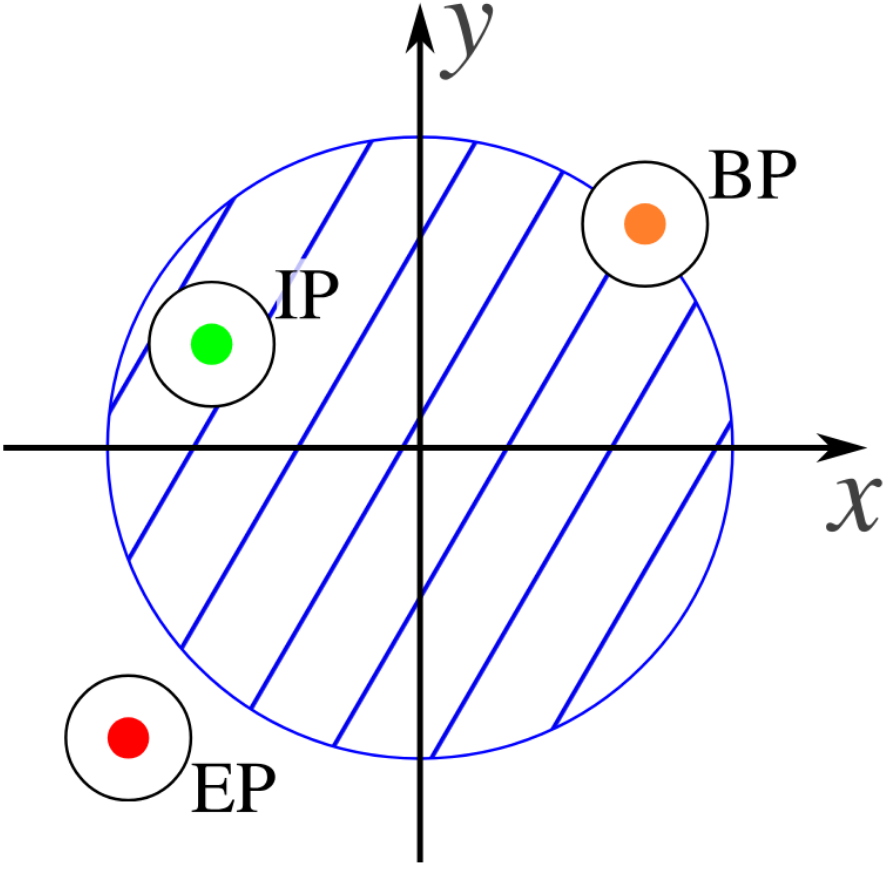
\includegraphics[width=0.5\textwidth]{ball.png}
	\caption{Interior point (IP), exterior point (EP), and boundary point (BP).}
	\label{fig:ball}
\end{figure}
Now that we have defined completeness, let us look at the difference between open and closed sets, particularly on the 2D plane. We will be considering a ball in the 2D plane,
defined,
\begin{Definitions}{Ball}{}
	A ball of radius $\epsilon$ around a point $\vb{r}_0$ is the set of all points $\vb{r}$ such that $\norm{\vb{r} - \vb{r}_0}$.
\end{Definitions} 
A sphere is the points where $\norm{\vb{r} - \vb{r}_0} = \epsilon$. Let us denote the set of the sphere $S$. We will consider three types of points, visualised in figure \ref{fig:ball},
\begin{itemize}
	\item \textbf{Exterior point}, for some $\epsilon$, all  $\vb{r} \notin S$.
	\item \textbf{Interior point}, for some $\epsilon$, all $\vb{r} \in S$.
	\item \textbf{Boundary point}, for some $\epsilon$, some of the neighbourhood of $\vb{r} \in S$ and some $\vb{r} \notin S$.
\end{itemize}
We can then define closed and open sets.
\begin{Definitions}{Closed Set}{}
	A set that contains all its boundary points is closed.
\end{Definitions}
An example of this is a set of points $\abs{r} \leq 1$, as $|r| = 1$ is a boundary point, and also belongs to the set. 
\begin{Definitions}{Open Set}{}
	A set that only includes interior points is open.
\end{Definitions}
We must furthmore define,
\begin{Definitions}{Connected Set}{}
	Sets for which any two points can be joined by a continuous path. 
\end{Definitions}
If a set is connected and open, we call it a \textit{region}.
\begin{Examples}{}{}
	The function $f(z) = \frac{1}{(1-z)}$ has a defined Taylor series for $z \neq 1$,
	\begin{equation}
		f(z) = \sum_{i=0}^{\infty}z^i.
	\end{equation}
	For what complex numbers is this series Cauchy? Is this an open or closed set?
\end{Examples}
We will consider the cases $|z| < 1$ and $|z| > 1$ separately, with $|z| =1$ as a boundary case. Let us define,
\begin{equation}
	a_n = \sum_{i=0}^n z^i.
\end{equation}
For any $z \neq 1$, assuming $n > m$,
\begin{equation}
	\abs{a_n - a_m} = \abs{\sum_{i = m+1}^n z_i } = \abs{\frac{z^{m+1}-z^{n+1}}{1-z}}.
\end{equation}
For $|z| < 1$,
\begin{equation}
	|a_n - a_m| = \frac{|z|^m}{|1-z|}\abs{1 - z^{n-m+1}}\leq \frac{2}{|1-z|}|z|^m
\end{equation}
and since $|z|^m$ is decreasing as a function of $m$, the series is Cauchy. For $|z|>1$,
\begin{equation}
	|a_n - a_m| = \frac{|z|^n}{|1-z|}\abs{1 - z^{-n+m+1}}\geq \frac{2}{|1-\frac{1}{z}|}|z|^n = z^{n+1}
\end{equation}
and since $|z|^{n}$ is an increasing function of $n$, the series is not Cauchy. Thus the series is Cauchy in the open set $|z| < 1$.
\section{Inner Product Space}
An inner product space is a vector space with an inner product, which is a generalisation of the scalar product.
\begin{Definitions}{Inner product, $\innerproduct{\vb{a}}{\vb{b}}$}{}
	Given a vector space $V_N$ over $\mathbb{F}$, the inner product between two vectors $\vb{a},\vb{b} \in V_N$ is a function such that $V \times V \to \mathbb{F}$. If $\mathbb{F} \subset \mathbb{C}$, the following properties hold,
	\begin{enumerate}
		\item \textbf{Linearity}. If $\vb{w} = \lambda\vb{u} + \mu\vb{v}$ then $\innerproduct{\vb{a}}{\vb{w}} = \lambda\innerproduct{\vb{a}}{\vb{u}} + \mu \innerproduct{\vb{a}}{\vb{u}}$.
		\item \textbf{Conjugation Symmetry.} $\overline{\innerproduct{\vb{w}}{\vb{a}}} = \innerproduct{\vb{a}}{\vb{w}}$
		\item \textbf{Positive Definiteness.} $\forall \vb{x}\neq0, \innerproduct{\vb{x}}{\vb{x}} > 0$.
	\end{enumerate}
\end{Definitions}
From our definition of the inner product, we can define the 2-norm,
\begin{equation}
	\norm{\vb{a}}^2 = \innerproduct{\vb{a}}{\vb{a}} \geq 0.
\end{equation}
\subsection{Orthogonality}
\begin{Definitions}{Orthogonality}{}
	$\forall \vb{a},\vb{b} \neq 0 \in V_N$ if $\innerproduct{\vb{a}}{\vb{b}} = 0$ then $\vb{a}$ and $\vb{b}$ are orthogonal.
\end{Definitions}
This allows us to then define an orthonormal basis.
\begin{Definitions}{Orthonormal basis}{}
	The set basis vectors $\left\{\vb{e}_i\right\}_{i=1}^N \in V_N$ is orthogonal if,
	\begin{equation}
		\innerproduct{\vb{e}_i}{\vb{e}_j} = A_i\delta_{ij}.
	\end{equation}
	and $A_i \neq 0$. The set of basis vectors is orthonormal for $A_i = 1, \forall i \in \left[1,N\right]$.
\end{Definitions}
Given we can decompose any vector $\vb{a} \in V_N$ if given a complete set of basis vectors, we can define a general inner product for $V_N$ over $\mathbb{F} \subset \mathbb{C}$. Let us begin by writing the decomposition of two vectors $\vb{a},\vb{b}\in V_N$ into a set of basis vectors $\left\{\vb{e}_j\right\}_{j=1}^N$,
\begin{align}
	\vb{a} = \sum_{j=1}^Na_j\vb{e}_j && \vb{b} = \sum_{j=1}^Nb_j\vb{e}_j.
\end{align}
Then, using linearity,
\begin{equation}
	\begin{split}
		\innerproduct{\vb{a}}{\vb{b}} & = \sum_{j,k=1}^N\overline{a}_j \innerproduct{\vb{e}_j}{\vb{e}_k}b_k \\
		& = \sum_{i,j=1}^N\overline{a}_j\delta_{jk}b_k \\
		& = \sum_{j=1}^N\overline{a}_jb_j.
	\end{split}
\end{equation}
NOTE: This only holds when using an orthonormal basis.
\\\\
We can obtain further insight into the decomposition of a vector by considering the inner product,
\begin{equation}
	\begin{split}
		\vb{a} = \sum_{j=1}^Na_j\vb{e}_j \implies \innerproduct{\vb{e}_k}{\vb{a}} & = \sum_{j=1}^Na_j\underbrace{\innerproduct{\vb{e}_j}{\vb{e}_k}}_{\delta_{jk}} = a_k.
	\end{split}
\end{equation}
We often refer to $a_k = \innerproduct{\vb{e}_k}{\vb{a}}$ as the \textit{projection} of $\vb{a}$ onto $\vb{e}_k$ as it gives the component of $\vb{a}$ in the $\vb{e}_k$ direction.
\subsection{Gram-Schmidt Orthonormalisation}
\begin{Definitions}{Gram-Schmidt Algorithm}{}
	Given a basis $\left\{\vb{v}_j\right\}_{j=1}^N \in V_N$,
	\begin{itemize}
		\item[1.] Define
		\begin{equation}
			\vb{e}_1 = \frac{\vb{v}_1}{\norm{\vb{v}_1}}
		\end{equation}
		\item[2.] Define 
		\begin{align}
			\vb{u}_2 = \vb{v}_2 - \innerproduct{\vb{e}_1}{\vb{e}_2}\vb{e_1}
	&&
			\vb{e}_2 = \frac{\vb{u}_2}{\norm{\vb{u}_2}}
		\end{align}
		\item[\vdots]
		\item[m.] Define,
		\begin{equation}
			\vb{u}_m = \vb{v}_m - \sum_{j=1}^{m-1}\innerproduct{\vb{e}_j}{\vb{v}_m}\vb{e}_j
		\end{equation}
		thus,
		\begin{equation}
			\vb{e}_m = \frac{\vb{u}_m}{\norm{\vb{u}_m}}
		\end{equation}
	\end{itemize}
	up to $N$.
\end{Definitions}
The Gram-Schmidt process is able to take any set of basis vectors and turn it into a set of orthonormal basis vectors. The idea behind it is that given 2 vectors $\vb{v},\vb{u}$ such that $\norm{\vb{u}} = 1$, then we wish to define a vector $\vb{v}' = \vb{v} - \innerproduct{\vb{u}}{\vb{v}}\vb{u}$. The inner product with $\vb{u}$ and this new vector is then,
\begin{equation}
	\innerproduct{\vb{u}}{\vb{v}'} = \innerproduct{\vb{u}}{\vb{v}} - \innerproduct{\vb{u}}{\vb{v}}\cancelto{1}{\innerproduct{\vb{u}}{\vb{u}}} = 0.
\end{equation}
So, we essentially are removing the non-orthonormal components from each subsequent basis vector, based on the first basis vector in the set.
\subsection{Inequalities of Inner Product Space}
\begin{Theorems}{Cauchy-Schwartz Inequality}{}
	$\forall \vb{a},\vb{b} \in V_N, \abs{\innerproduct{\vb{a}}{\vb{b}}} \leq \norm{\vb{a}}\norm{\vb{b}}$.
\end{Theorems}
\begin{proof}
	Consider $\vb{u} = \vb{a} - \lambda\vb{b}$,
	\begin{equation}
		\norm{\vb{a}}^2 = \norm{\vb{a}}^2 + |\lambda|^2\norm{\vb{b}}^2 - \overline{\lambda}\innerproduct{\vb{b}}{\vb{a}} - \lambda\innerproduct{\vb{a}}{\vb{b}} \geq 0.
	\end{equation}
Choose, 
\begin{equation}
	\lambda = \frac{\innerproduct{\vb{b}}{\vb{a}}}{\norm{\vb{b}}^2}.
\end{equation}
Thus,
\begin{equation}
	\begin{split}
		\norm{\vb{u}}^2 = \norm{\vb{a}}^2 \norm{\vb{b}}^2 - \frac{\abs{\innerproduct{\vb{a}}{\vb{b}}}}{\norm{\vb{b}}^2} \geq 0
	\end{split}
\end{equation}
$\implies \abs{\innerproduct{\vb{a}}{\vb{b}}} \leq \norm{\vb{a}}\norm{\vb{b}}$.
\end{proof}
\begin{Theorems}{Triangle Inequality}{}
	$\forall \vb{a},\vb{b} \in V_N, \norm{\vb{a} + \vb{b}}  \leq \norm{\vb{a}} + \norm{\vb{b}}$
\end{Theorems}
\begin{proof}
	\begin{equation}
		\begin{split}
		\norm{\vb{a} + \vb{b}}^2 & = \innerproduct{\vb{a} + \vb{b}}{\vb{a} + \vb{b}} \\
		& \leq \norm{\vb{a}}^2 + \norm{\vb{b}}^2 + 2\abs{\innerproduct{\vb{a}}{\vb{b}}} \\
		& \leq \norm{\vb{a}}^2 + \norm{\vb{b}}^2 + 2\norm{\vb{a}}\norm{\vb{b}} = (\norm{\vb{a}} + \norm{\vb{b}})^2
		\end{split}
	\end{equation}
	$\implies \norm{\vb{a} + \vb{b}} \leq \norm{\vb{a}} + \norm{\vb{b}}$
\end{proof}
\section{Function Space}
We denote function spaces by $\mathcal{F}$. Let us define the function space inner product.
\begin{Definitions}{Function Space Inner Product}{}
	For $x \in \left[a,b\right]$, and functions $f,g : \left[a,b\right] \to \mathbb{C}$, the inner product is given by
	\begin{equation}
		\braket{f}{g} = \int_a^b\overline{f(x)}g(x)\dd\mu(x)
	\end{equation}
	where $\dd\mu(x)$ is the integration measure of a function space.
\end{Definitions}
The inner product must satisfy,
\begin{equation}
	\norm{f}^2 = \braket{f}{f} = \int_a^b |f(x)|^2\dd\mu(x) \geq 0
\end{equation}
which is only 0 if $f(x) = 0 \forall x$. If $\norm{f}^2$ is finite, then $f$ is square-integrable and can be normalised. Function spaces where all functions are square-integrable are known as Hilbert spaces.
\begin{Definitions}{L2 Functions}{}
	A function $f$ is said to be in the space $L^2(\left[a,b\right])$ if $\norm{f}^2 = \int_a^b|f(x)|^2\dd\mu(x) < \infty$.
\end{Definitions}
Let us note that we will use $\dd\mu(x) = \dd{x}$ throughout the course, however most concepts can be generalised to an arbitrary measure.
\subsection{Basis functions and completeness}
A function $f \in \mathcal{F}$ over the domain $x \in \left[a,b\right]$ can be represented by a set of basis vectors $\left\{u_n\right\}_{n=1}^{\infty} \in \mathcal{F}$ as,
\begin{equation}
	f(x) = \sum_{n=1}^{\infty}f_nu_n(x)
\end{equation}
where the coefficients $f_n$ are defined,
\begin{equation}
	f_n = \braket{u_n}{f} = \int_a^b\overline{u_n(x)}f(x)\dd{x}.
\end{equation}
We can define the completeness relation for an infinite function space by,
\begin{equation}
	\sum_{n=1}^{\infty}u_n(x) \overline{u_n(y)} = \delta(x-y).
\end{equation}
\subsection{Coordinate Representation}
When we write $f(x)$, we are referring to a function $f \in \mathcal{F}$ in a basis defined by the coordinate $x$. Let us write this more explicitly, calling $\ket{x}$ the \textit{position vector}, and writing $f \in \mathcal{F}$,
\begin{equation}
	\ket{f} = \int_a^b\dd{x}f(x)\ket{x}
\end{equation}
where we integrate rather than sum since position is continuous. We can then clearly see,
\begin{equation}
	f(x) = \braket{x}{f} = \int_a^b\delta(y-x)f(y)\dd{y}
\end{equation}
from which we find that the Dirac-delta acts as a basis vector for position vectors. We define the overlap of two position vectors,
\begin{equation}
	\braket{x}{x'} = \int_a^b\delta(y-x)\delta(y-x')\dd{y} = \delta(x-x') \iff x,x'\in\left[a,b\right].
\end{equation}
The completeness relation is then,
\begin{equation}
	\int_a^b\ket{x}\bra{x}\dd{x} = \hat{\mathbb{1}}.
\end{equation}
\chapter{Linear Operators}
\begin{Definitions}{Map}{}
	A map $M$ is a function which takes $V \to W$ where $V,W$ are vector spaces. This is such that $M$ acting on $\vb{c} \in V$ produces a different vector $\vb{c}' \in W$.
\end{Definitions}
We are often interested in linear maps, or linear operators as they are often called in physics.
\begin{Definitions}{Linear Operator}{}
	An operator $\hat{A}$ is linear if, for a vector $\vb{c} = \lambda \vb{a} + \mu\vb{b}$ where $\forall \lambda, \mu \in \mathbb{F}$ and $\forall \vb{a},\vb{b} \in V$ over $\mathbb{F}$, 
	\begin{equation}
		\vb{c}' = \hat{A}\vb{c} = \mu(\hat{A}\vb{a})+ \lambda (\hat{A}\vb{b})
	\end{equation}
\end{Definitions}
In physics, but not generally, linear operators always map $V \to V$.
\section{Algebra of operators}
We can define the following properties of linear operators,
\begin{enumerate}
	\item $(\hat{A} + \hat{B}) \equiv \hat{A}\vb{v} + \hat{B} \vb{v}$.
	\item $(\lambda\hat{A})\vb{v} = \lambda(\hat{A}\vb{v})$.
	\item $\exists\hat{\mathbb{1}} : \hat{\mathbb{1}}\vb{v} = \vb{v}, \forall \vb{v} \in V$.
	\item $\exists \hat{0} : \hat{0}\vb{v} = \vb{0}, \forall \vb{v} \in V$.
	\item $\forall \vb{v} \in V, (\hat{B}\hat{A})\vb{v} = \hat{B}(\hat{A}\vb{v})$, generally $\hat{A} \hat{B} \neq \hat{B}\hat{A}$
\end{enumerate}
\section{Matrix Representation of Linear Operators}
Consider $V_N$ over $\mathbb{F}$. Assume $\left\{\vb{e}_j\right\}_{j=1}^N$ is an orthonormal basis. $\forall \vb{v} \in V_N$,
\begin{equation}
	\vb{v} = \sum_{j=1}^Nv_j \vb{e}_j
\end{equation}
where $\innerproduct{\vb{e}_k}{\vb{v}} = v_k$. Given a linear operator $\hat{A}$,
\begin{equation}
	\hat{A} \vb{v} = \hat{A} \left(\sum_{j=1}^N v_j\vb{e}_j\right) = \sum_{j=1}^Nv_j\hat{A}\vb{e}_j
\end{equation}
by linearity. We have $\hat{A}\vb{e}_j \in V_N$, thus,
\begin{equation}
	\hat{A} \vb{e}_j = \sum_{i=1}^N\vb{e}_i\underbrace{(\hat{A}\vb{e}_j)}_{A_{ij}}
\end{equation}
so,
\begin{equation}
	\begin{split}
		& \hat{A}\vb{e}_j = \sum_{i=1}^N\vb{e}A_{ij} \\
		\implies & A_{ij} = \innerproduct{\vb{e}_i}{\hat{A}\vb{e}_j}.
	\end{split}
\end{equation}
So,
\begin{equation}
	\begin{split}
		\hat{A}\vb{v} & = \sum_{j=1}^Nv_j\sum_{i=1}^N(A_ij\vb{e}_i) \\
		& =\sum_{i=1}^{N}\left(\sum_{j=1}^NA_{ij}v_j\right)\vb{e}_i
	\end{split}
\end{equation}
thus,
\begin{equation}
	(\hat{A}\vb{v})_i = \sum_{j=1}^N A_{ij}v_j.
\end{equation}
Interestingly, we have obtained matrix multiplication from linearity and orthonormality, rather than having to define it.
\section{Inverse Operator}
\begin{Definitions}{Inverse operator}{}
	Given an operator $\hat{A}$ from $V \to V$, $\forall \vb{v} \in V$, $\exists \hat{B}$ such that, $\hat{B}(\hat{A}\vb{v}) = \vb{v}$, $(\hat{B}\hat{A})\vb{v} = \vb{v} \implies \hat{B}\hat{A} = \hat{\mathbb{1}}$. We call $\hat{B} = \hat{A}^{-1}$.
\end{Definitions}
NOTE: Not all operators have an inverse.
\section{Dyadic (Outer) Product}
Recall $\bra{u}\hat{A}\ket{v} \to$ $\vb{u}^{\dag}\hat{A}\vb{v}$, or $\innerproduct{\vb{u}}{\hat{A}\vb{v}}$. We can clearly see that $\vb{c}\innerproduct{\vb{a}}{\vb{b}}$ is a vector. Let us define,
\begin{equation}
	\vb{c}' = \vb{c}(\vb{a}^{\dag}\vb{b}) = \underbrace{(\vb{c}\vb{a}^{\dag})}_{\substack{\text{Linear}\\\text{Operator}}}\vb{b}
\end{equation}
this linear operator is known as a \textit{dyad} or the \textit{outer product} of $\vb{a}$ and $\vb{c}$. Let us define it more formall,y

\begin{Definitions}{Dyad/Outer product}{}
	For $V_N \subset \mathbb{C}^N$, and vectors $\vb{a},\vb{b} \in V_N$, their outer product is defined $\vb{a}\vb{b}^{\dag}$. It has the following properties,
	\begin{enumerate}
		\item \textbf{Linearity in the first argument}. If $\vb{c} = \lambda \vb{a} + \mu \vb{b}$, then $\vb{c}\vb{d}^{\dag} = \lambda\vb{a}\vb{d}^{\dag} + \mu\vb{b}\vb{d}^{\dag}$.
		\item \textbf{Antilinearity in the second argument}. If $\vb{d} = \lambda \vb{a} + \mu \vb{b}$, then $\vb{c}\vb{d}^{\dag} = \bar{\lambda}\vb{c}\vb{a}^{\dag} + \bar{\mu}\vb{c}\vb{b}^{\dag}$.
	\end{enumerate}
\end{Definitions}
\section{Projection Operator and the Completeness Relation}
If $\hat{P}^2\vb{v} = \hat{P}\vb{v}$, $\forall \vb{v} \in V_N$, then $\hat{P}$ is a projection operator. For a given orthonormal basis $\left\{\vb{e}_j\right\}_{j=1}^N \in V_N$, $\hat{P}_j = \vb{e}_j\vb{e}_j^{\dag}$. A consequence of this is the completeness relation, 
\begin{equation}
	\sum_{j=1}^N\hat{P}_j = \sum_{j=1}^N \vb{e}_j\vb{e}_j^{\dag} = \hat{\mathbb{1}}.
\end{equation}
\section{The Adjoint or Hermitian Conjugate}
\begin{Definitions}{Adjoint}{}
	\begin{equation}
	\forall \hat{A}, \forall \vb{u},\vb{v} \in V_N : \innerproduct{\vb{u}}{\hat{A}^{\dag}\vb{v}} = \overline{\innerproduct{\vb{v}}{\hat{A}\vb{u}}}
\end{equation}
In matrix notation,
\begin{equation}
	(\hat{A}^{\dag})_{ij} = \overline{A_{ji}}.
\end{equation}
An operator is self adjoint if $\hat{A} = \hat{A}^{\dag}$.
\end{Definitions}
\begin{Definitions}{Unitary Operator}{}
	\begin{equation}
		\exists \hat{U} : \hat{U}^{\dag}\hat{U} = \hat{U}\hat{U}^{\dag} = \hat{\mathbb{1}}
	\end{equation}
	i.e.,
	\begin{equation}
		\hat{U}^{-1} = \hat{U}^{\dag}.
	\end{equation}
\end{Definitions}

\section{Representations}
\subsection{Representation of a Vector}
We know that a vector can be decomposed into orthonormal basis vectors. A vector space can have more than one set of orthonormal basis vectors which can represent a given vector. From the completeness relation, we find,
\begin{equation}
	\begin{split}
		\vb{v} = \hat{\mathbb{1}}\vb{v} &= \sum_{j=1}^N \innerproduct{\vb{e}_j}{\vb{v}}\vb{e}_j \\ 
		& = \sum_{j=1}^N\innerproduct{\vb{f}_j}{\vb{v}}\vb{f}_j
	\end{split}
\end{equation}
i.e., changing basis does not change the abstract concept of a vector.
\subsubsection{Invariance of the Inner Product}
We can emphasise the idea above by considering the inner product of a vector. We can write some vector $\vb{v}\in V_N$ as,
\begin{equation}
	\vb{v} = \sum_{j=1}^Na_i\vb{e}_i = \sum_{j=1}^N b_i\vb{f}_i.
\end{equation}
Computing the inner product,
\begin{equation}
	\begin{split}
	\innerproduct{\vb{v}}{\vb{v}} & = \sum_{j=1}^N\left(a_j\vb{e}_j\right)^{\dag}\sum_{k=1}^Na_k\vb{e}_k \\
	& = \sum_{j=1}^N\sum_{k=1}^N\overline{a_j}a_k\underbrace{\vb{e}_j^{\dag}\vb{e}_k}_{\delta_{jk}} \\
	& = \sum_{j=1}^N\abs{a_j}^2
	\end{split}
\end{equation}
and repeating this using the $\left\{\vb{f}_j\right\}_{j=1}^N$ representation,
\begin{equation}
	\begin{split}
		\innerproduct{\vb{v}}{\vb{v}} & = \sum_{j=1}^N\left(b_j\vb{f}_j\right)^{\dag}\sum_{k=1}^Nb_k\vb{f}_k \\
		& = \sum_{j=1}^N\abs{b_j}^2
	\end{split}
\end{equation}
and we find $\sum_{j=1}^N\abs{a_j}^2 = \sum_{j=1}^N\abs{b_j}^2$, so the inner product is invariant under a basis change.
\subsection{Representation of Linear Operators}
Consider a vector space $V_N$ with basis $\left\{\vb{e}_j\right\}_{j=1}^N$. Consider $\vb{b},\vb{c} \in V_N$ and an operator $\hat{A}$, such that $\vb{c} = \hat{A}\vb{b}$. We can find its representation by considering,
\begin{equation}
	\begin{split}
		\mathbb{1} \vb{c} = \mathbb{1} \hat{A}\mathbb{1}\vb{b} & \\
		\sum{j=1}^N \innerproduct{\vb{e}_j}{\vb{c}} \vb{e}_j & = \sum_{j,k=1}^N\left(\vb{e}_j\vb{e}_j^{\dag}\right)\hat{A}\left(\vb{e}_k\vb{e}_k^{\dag}\right)\vb{b} \\
		& = \sum_{j,k=1}^N \vb{e}_j\underbrace{\left(\vb{e}_j^{\dag}\hat{A}\vb{e}_k\right)}_{A_{ij}}\underbrace{\left(\vb{e}_k^{\dag}\vb{b}\right)}_{b_k}
	\end{split}
\end{equation}
Thus, we find that we can denote the entries of a matrix $\doubleunderline{A}$ representing a linear operator $\hat{A}$ are $\left(\doubleunderline{A}\right)_{ij}$. We can denote this representation by,
\begin{align}
	\hat{A} \xrightarrow{\left\{\vb{e}\right\}_{j=1}^N} \doubleunderline{A}.
\end{align}
\subsection{Changing Representation of a Vector}
Consider a vector $\vb{v} \in V_N$, and orthonormal bases $\left\{\vb{e}_j\right\}_{j=1}^N$ and $\left\{\vb{f}_j\right\}_{j=1}^N$. $\vb{v}$ can be decomposed as,
\begin{equation}
		\vb{v} = \sum_{j=1}^Na_i\vb{e}_i = \sum_{j=1}^N b_i\vb{f}_i.
\end{equation}
The $l^{\text{th}}$ element of the vector is given by,
\begin{equation}
	a_l = \innerproduct{\vb{e}_l}{\vb{v}} = \sum_{k=1}^Nb_k\innerproduct{\vb{e}_l}{\vb{f}_k} = \sum_{k=1}^N\left(\doubleunderline{U}_{lk}\right)b_k
\end{equation}
where we have found the matrix $(\doubleunderline{U})_{lk}$ which represents a unitary operator that takes a vector representation from one basis and transforms it into another. We can denote this,
\begin{equation}
	\begin{pmatrix}
		a_1 \\ a_2 \\ \vdots \\ a_N
	\end{pmatrix} = \begin{pmatrix}
	\innerproduct{\vb{e}_1}{\vb{f}_1} & \cdots & \innerproduct{\vb{e}_1}{\vb{f}_N} \\
	\innerproduct{\vb{e}_2}{\vb{f}_1} & \cdots & \innerproduct{\vb{e}_2}{\vb{f}_N} \\
	\vdots & \ddots & \vdots \\
	\innerproduct{\vb{e}_N}{\vb{f}_1} & \cdots & \innerproduct{\vb{e}_N}{\vb{f}_N}
	\end{pmatrix}\begin{pmatrix}
	b_1 \\ b_2 \\ \vdots \\ b_N
	\end{pmatrix}
\end{equation} 
\subsection{Changing Representation of a Matrix}
We can write a linear operator as,
\begin{equation}
	\hat{A} = \mathbb{1}\hat{A} \mathbb{1} = \sum_{j,k=1}^NA_{jk}\vb{e}_j\vb{e}_k^{\dag} = \sum_{l,m=1} \tilde{A}_{lm}\vb{f}_l\vb{f}_m^{\dag}
\end{equation}
we then find that,
\begin{equation}
	A_{jk} = \sum_{l,m=1}^N \innerproduct{\vb{e}_j}{\vb{f}_l}\tilde{A}_{lm}\innerproduct{\vb{f}_m}{\vb{e}_k}.
\end{equation}
Thus, we find that we can change the matrix representation of a linear operator by,
\begin{equation}
	\doubleunderline{A} = \doubleunderline{U}\doubleunderline{\tilde{A}}\doubleunderline{U}^{\dag}.
\end{equation}
\section{Eigenvalue Problems}
\begin{Definitions}{Eigen Equation}{}
	For a linear operator $\hat{A}$, the eigenequation is,
	\begin{equation}
		\hat{A}\vb{u}= \lambda \vb{u}
	\end{equation}
	where $\lambda$ and $\vb{u}$ are the eigenvalue and right eigenvector of $\hat{A}$ respectively, such that $\vb{u} \neq \vb{0}$.
\end{Definitions}
A left eigenvector will satisfy,
\begin{equation}
	\vb{v}^{\dag}\hat{A} = \lambda\vb{v}^{\dag}.
\end{equation}
In order to obtain the eigenvalues, we rearrange to get,
\begin{equation}
	\left(\hat{A} - \lambda \hat{\mathbb{1}}\right)\vb{u} = 0
\end{equation}
and solve,
\begin{equation}
	\det\left(\hat{A} - \lambda \hat{\mathbb{1}}\right)
\end{equation}
which generates a polynomial of degree $N$, with $N$ solutions for $\lambda in \mathbb{C}$. Each distinct eigenvalue will correspond to a distinct eigenvector. However, if we have a repeated root, we get repeated eigenvectors. For $m > 1$ repeated eigenvectors, there may be up to, but at least 1, $m$ linearly independent eigenvectors corresponding to the degenerate eigenvalue. 
\subsection{Eigenvalues and eigenvectors of Hermitian operators}
\begin{Theorems}{Eigenvalues of Hermitian Operators}{}
	Consider the eigenvalues $\left\{\lambda_i\right\}_{i=1}^N$ and eigenvectors $\left\{\vb{u}\right\}_{i=1}^N$ of $\hat{A}$. $\forall \hat{A} : \hat{A}^{\dag} = \hat{A} \implies \forall i: \lambda_i \in \mathbb{R}$, $\forall i\neq j: \vb{u}_i^{\dag}\vb{u}_j = 0$.
\end{Theorems}
\begin{proof}
	The eigenvalue equation is given by,
	\begin{equation}
		\hat{A}\vb{u}_i = \lambda_i \vb{u}_i.
	\end{equation}
	Without loss of generality, consider the matrix elements of $\hat{A}$ with respect to two eigenvectors,
	\begin{equation}
		\vb{u}_j^{\dag}\hat{A}\vb{u}_k = \lambda_k\innerproduct{\vb{u}_j}{\vb{u}_k}. \label{eq:1}
	\end{equation}
	Using the Hermitian property,
	\begin{equation}
		\vb{u}_j^{\dag}\hat{A}\vb{u}_k = \vb{u}_j^{\dag}\hat{A}^{\dag}\vb{u}_k = \overline{\vb{u}_k^{\dag}\hat{A}\vb{u}_j} = \overline{\lambda_j}\left<\vb{u}_j, \vb{u}_k\right>. \label{eq:2}
	\end{equation}
	Equating equations \eqref{eq:1} and \eqref{eq:2},
	\begin{equation}
		(\lambda_k - \overline{\lambda}_k)\innerproduct{\vb{u}_j}{\vb{u}_k} = 0.
	\end{equation}
	Let us consider two cases,
	\begin{enumerate}
		\item $k = j$, since $\innerproduct{\vb{u}_j}{\vb{u}_j} > 0$, we require $\lambda_j = \overline{\lambda}_j$. 
		\item $k\neq j$, since $\lambda_j, \lambda_k$ are distinct, we require $\innerproduct{\vb{u}_j}{\vb{u}_k} = 0$. 
	\end{enumerate}
\end{proof}
\subsection{Diagonalisation}
Let $\doubleunderline{U}$ be the matrix with orthonormal eigenvectors $\vb{u}_j$ as columns, such that $U_{ij} = (u_j)_i$, and $\hat{U}$ be the corresponding linear operator. By orthogonality, $\hat{U}$ is unitary. For a linear operator $\hat{A}$, we can diagonalise it (construct a matrix with $\hat{A}$'s eigenvalues on the diagonal) by,
\begin{equation}
	\left[\hat{U}^{\dag}\hat{A}\hat{U}\right]_{ij} = \lambda_i\delta_{ij}.
\end{equation}
To obtain the original operator form its diagonalised form $\Lambda_{ij}$, we perform,
\begin{equation}
	A_{ij} = U_{ik}\Lambda_{kl}\overline{U}_{jl}.
\end{equation}
\subsubsection{Eigenvalues and eigenvectors of unitary operators}
We use unitary operators in physics to describe time evolution in quantum mechanics. We can do this because they preserve the norm, and thus the inner product, of a vector. i.e., $\innerproduct{\hat{U}\vb{u}}{\hat{U}\vb{v}} = \innerproduct{\vb{u}}{\vb{v}}$.
\begin{Theorems}{Eigenvalues of unitary operators}{}
	Consider a unitary operator $\hat{U} : V \to V$ with eigenvalue equation,
	\begin{equation}
		\hat{U}\vb{u}_j = \lambda_j\vb{u}_j.
	\end{equation}
	The eigenvalues satisfy the following condition:
	\begin{enumerate}
		\item $\abs{\lambda_j} = 1 \implies \lambda_j = e^{i\theta_j}, \theta \in \mathbb{R}$.
		\item $\lambda_j \neq \lambda_k \implies \innerproduct{\vb{u}_j}{\vb{u}_k} = 0$.
		\item The eigenvectors of $\hat{U}$ form an orthonormal basis for $V$.
	\end{enumerate}
\end{Theorems}
\begin{proof}
	\begin{enumerate}
		\item We need to prove that $\abs{\lambda_j}^2 = 1$. Consider the left anr right eigenequations of $\hat{U}$,
		\begin{align}
			\hat{U}\vb{u}_j &= \lambda\vb{u}_j\\
			\vb{u}_j^{\dag}\hat{U}^{\dag} & = \overline{\lambda_j} \vb{u}_j^{\dag}
		\end{align}
		from which we find,
		\begin{equation}
			\begin{split}
			\vb{u}_j^{\dag}\hat{U}^{\dag}\hat{U}\vb{u}_j & = \vb{u}^{\dag}\hat{\mathbb{1}}\vb{u} = \overline{\lambda}\lambda\vb{u}^{\dag}_j\vb{u}_j \\
			& = \vb{u}^{\dag}\vb{u} = |\lambda|^2\vb{u}_j^{\dag}\vb{u} \\
			& \implies \left(1 - |\lambda|^2\right)\vb{u}^{\dag}_j\vb{u}_j
			\end{split}
		\end{equation}
		we have $\vb{u} \neq \vb{0}$, so we require $|\lambda|^2 = 1$, and thus $\lambda = e^{i\theta}, \theta \in \mathbb{R}$.
		\item Let us consider the left and right eigenequations again. We have,
		\begin{equation}
			\begin{split}
				\vb{u}_j^{\dag}\vb{u}_k & = \overline{\lambda_j}\lambda_k\vb{u}_j^{\dag}\vb{u}_k \\
				\implies \innerproduct{\vb{u}_j}{\vb{u}_k}(1 - \overline{\lambda_j}\lambda_k) & = 0
			\end{split}
		\end{equation}
		we require $\overline{\lambda_j}\lambda_k \neq 1, \forall j \neq k, \therefore \innerproduct{\vb{u}_j}{\vb{u}_k}$.
		\item For completeness, we must write $\vb{v} = \sum_{j=1}^Nc_j\vb{u}_j$. We have shown $\left\{\vb{u}_j\right\}_{i=1}^N$ to be orthonormal, so we can write,
		%\begin{equation}
			$c_j = \innerproduct{\vb{u}_j}{\vb{v}}$.
		%\end{equation}
	\end{enumerate}
\end{proof}
\subsubsection{Spectral Representation}
We can diagonalise a general operator $\hat{A}$ which is not necessarily Hermitian, under the assumption that it has a complete set of eigenvectors. The left and right eigenvector equations are,
\begin{align}
	\vb{v}_j^{\dag}\hat{A} = \lambda_j\vb{v}_j^{\dag} && \hat{A}\vb{u}_j = \lambda_j\vb{u}_j.
\end{align}
We then have,
\begin{equation}
	\vb{v}_j^{\dag}\hat{A}\vb{u}_k = \lambda_k\innerproduct{\vb{v}_j}{\vb{u}_k} = \lambda_j\innerproduct{\vb{v}_j}{\vb{u}_k}
\end{equation}
thus for $\lambda_j \neq \lambda_k$, we require $\innerproduct{\vb{v}_j}{\vb{u}_k} = 0$.
\\\\
We choose a normalisation $\innerproduct{\vb{v}_j}{\vb{u}_k}$, the completeness relation is given by,
\begin{equation}
	\sum_{j=1}^N \vb{u}_j\vb{v}_j^{\dag} = \hat{\mathbb{1}}
\end{equation}
and we call $\vb{v}_j$ the dual basis to $\vb{u}_j$. We can thus write the operator $\hat{A}$,
\begin{equation}
	\boxed{\hat{A} = \hat{A}\hat{\mathbb{1}} = \sum_{j=1}^N\hat{A}\vb{u}_j\vb{v}_j^{\dag} = \sum_{j=1}^N\lambda_j\vb{u}_j\vb{v}_j^{\dag}}
\end{equation}
which is known as the \textit{spectral representation} of $\hat{A}$. Given an orthonormal basis $\left\{\vb{e}_j\right\}_{j=1}^N$ in which we can write the matrix representation of $\hat{A}$ which we denote $\doubleunderline{A}$, we can diagonalise it by applying,
\begin{equation}
	\doubleunderline{A}^{\text{diag}} = \doubleunderline{S} \doubleunderline{A} \doubleunderline{T}^{\dag}
\end{equation}
where we define,
\begin{align}
	\left(\doubleunderline{S}\right)_{jk} = \innerproduct{\vb{v}_j}{ \vb{e}_k} && \left(\doubleunderline{T}\right)_{jk} = \innerproduct{\vb{u}_j}{\vb{e}_k}
\end{align}
which are unitary only if $\hat{A}$ is Hermitian.
\subsubsection{Diagonalisation of commuting operators}
For two commuting operators $\hat{A}$ and $\hat{B}$, when,
\begin{equation}
	\hat{B} \vb{u} = \lambda \vb{u}
\end{equation}
we have,
\begin{equation}
	\begin{split}
		& \hat{A}\hat{B}\vb{u} = \lambda\hat{A}\vb{u} \\
		\implies & \hat{B}\hat{A} = \lambda \left(\hat{A}\vb{u}\right)
	\end{split}
\end{equation}
and thus $\hat{A}\vb{u}$ is also an eigenvector of $\hat{B}$ with eigenvalue $\lambda$. Below the implications of this statement are stated,
\begin{itemize}
	\item \textbf{Non-degenerate:} If $\lambda$ is non-degenerate, $\forall\lambda, \exists\vb{u} : \hat{A}\vb{u} = \mu\vb{u} \implies$ $\vb{u}$ is a simultaneous eigenvector of $\hat{B}$ and $\hat{A}$.
	\item \textbf{Degenerate:} If $\lambda$ has degeneracy $m > 1$, with eigenvectors $\left\{\vb{u}_j\right\}_{j=1}^m$, then a linear combination of these eigenvectors is an eigenvector of $\hat{A}$. $\hat{B}$ will act in this subspace, and it is possible to find a basis which simultaneously diagonalises $\hat{A}$ and $\hat{B}$.
\end{itemize}
\section{Functions of Operators}
We wish to apply functions such as $\exp(\hat{A})$ to linear operators, and more generally functions such as $f$. 
\subsection{Taylor Expansion about 0}
We have well defined multiplication and addition on operators, so we can construct a Taylor series to define a function of an operator in most cases.
\begin{Definitions}{$f(\hat{A})$}{}
	For $f : \mathbb{C} \to \mathbb{C}$, with a Taylor series about $0$,
	\begin{equation}
		f(z) = \sum_{n=0}^{\infty}\frac{f^{(n)}(0)}{n!}z^n
	\end{equation}
	we define the composition of the function and an operator $\hat{A}$ by the same series,
	\begin{equation}
		f(\hat{A}) = \sum_{n=0}^{\infty}\frac{f^{(0)}}{n!}\hat{A}^n.
	\end{equation}
\end{Definitions}
where,
\begin{align}
	f^{(n)}(0) = \eval{\dv[n]{f(0)}{x}}_{0} && \hat{A}^n = \underbrace{\hat{A}\hat{A}\ldots\hat{A}}_{n\text{ times}}
\end{align}
\subsection{Spectral Decomposition}
Given $\hat{A}$ is diagonalisable, let us apply $f(\hat{A})$ to an eigenvector $\vb{u}$ of $\hat{A}$ with eigenvalue $\lambda$, assuming $f$ has a Taylor series,
\begin{equation}
	\begin{split}
		f(\hat{A})\vb{u} & = \sum_{n=0}^{\infty}\frac{f^{(n)}(0)}{n!}\hat{A}^n\vb{u} \\
		& = f(0) \vb{u} + \sum_{n=1}^{\infty}\frac{f^{(n)}(0)}{n!}\hat{A}^{n-1}\lambda^n\vb{u} \\
		& = \sum_{n=0}^{\infty}\frac{f^{(n)}(0)}{n!}\lambda^n\vb{u} = f(\lambda)\vb{u}.
	\end{split}
\end{equation}
If the eigenbasis of $\hat{A}$ is complete, we are able to work in it to represent $f(\hat{A})$ as,
\begin{equation}
	f(\doubleunderline{A}) = \text{diag}\left(\left\{f(\lambda_j)\right\}_{j=1}^N\right)
\end{equation}
where $\text{diag}$ is a function which constructs a matrix with the values in its arguments on the diagonal, and 0s in all other elements. We can then construct the final operator,
\begin{equation}
	f(\hat{A}) = \sum_{i=1}^Nf(\lambda_i) f(\lambda_i)\vb{u}_i\vb{v}_i^{\dag}
\end{equation}
where $\vb{v}_i^{\dag} = \vb{u}_i^{\dag}$ for a Hermitian operator.
\subsection{Time Evolution Operator}
\begin{Theorems}{Unitary operators as exponentials}{}
	For a Hermitian operator $\hat{A}$, then,
	\begin{equation}
		\hat{U}(\theta) = \exp(-i\hat{A}\theta) \label{eq:timeev}
	\end{equation}
	where $\theta \in \mathbb{R}$, is also unitary.
\end{Theorems} 
\begin{proof}
	Considering the spectral representation of $\hat{A}$, with eigenvalues $\lambda_j$ and eigenvectors $\vb{u}_j$, such that $\hat{A} = \sum_{j=1}^N\lambda_j\vb{u}_j\vb{u}_j^{\dag}$ then,
	\begin{equation}
		\hat{U}(\theta) = \sum_{j=1}^N\exp(-i\lambda_j\theta) \vb{u}_j\vb{u}_j^{\dag}.
	\end{equation}
	The adjoint $\hat{U}^\dag(\theta)$ is,
	\begin{equation}
		\hat{U}^{\dag}(\theta) = \sum_{j=1}^N\exp(i\lambda_j\theta) \vb{u}_j\vb{u}_j^{\dag}
	\end{equation}
	we then find,
	\begin{equation}
		\begin{split}
			\hat{U}^\dag(\theta)\hat{U}(\theta) & = \sum_{j,k}e^{-i(\lambda_j - \lambda_k)\theta}\vb{u}_k\vb{u}_k^{\dag}\vb{u}_j\vb{u}_j^{\dag} = \sum_{jk}e^{-i(\lambda_j - \lambda_k)\theta}\vb{u}_k^{\dag}\innerproduct{\vb{u}_k}{\vb{u}_j}\vb{u}_j \\
			& = \sum_{jk}e^{-i(\lambda_j - \lambda_k)\theta}\vb{u}_k^{\dag}\delta_{kj}\vb{u}_j = \sum_j \vb{u}_j\vb{u}_j^{\dag} = \hat{\mathbb{1}}.
		\end{split}
	\end{equation}
	thus the operator is unitary.
\end{proof}
Furthermore, the operator in equation \eqref{eq:timeev} is the time-evolution operator in quantum mechanics, where we would replace $\hat{A}$ with $\hat{H}$ and $\theta$ with $t$.
\subsection{Overlap Matrix}
We wish to develop an alternative method to the Gram-Schmidt process, and will allow us to generalise some things. Let us suppose we have a set of vectors $\left\{\vb{v}_j\right\}_{j=1}^M$ in a vector space $V_N$. We will \textbf{not} assume that $M \leq N$. The matrix overlap is given by,
\begin{equation}
	\hat{N} = \sum_{i=1}^M\vb{v}_i\vb{v}_i^{\dag}
\end{equation}
which is Hermitian, and whose matrix representation can be written,
\begin{equation}
	N_{kl} = \sum_{i=1}^Mv_{ik}\overline{v}_{il}.
\end{equation}
If we are given normalised eigenvectors $\vb{u}$ and eigenvalues of $\hat{N}$, we find,
\begin{equation}
	\vb{u}_k^{\dag}\hat{N}\vb{u}_k = \lambda_k = \sum_{i=1}^N\abs{\innerproduct{\vb{v}_i}{\vb{u}_k}}^2 \geq 0
\end{equation}
so, all of its eigenvalues must be either positive or 0. If all eigenvalues are positive, we find the inverse of the overlap matrix by writing it in the orthonormal basis $\left\{\vb{u}_j\right\}_{j=1}^M$,
\begin{equation}
	\hat{N}^{-1} = \sum_{i=1}^M\lambda_i^{-1}\vb{u}_i\vb{u}_i^{\dag}.
\end{equation}
For the case that we have a zero eigenvalue, we can define a \textit{pseudo-inverse}.
\begin{Definitions}{Pseudo-inverse}{}
	For a Hermitian operator $\hat{N}$ with a set of eigenvalues $\left\{\lambda_i\right\}_{i=1}^{M}$ and a set of normalised eigenvectors $\left\{\vb{u}\right\}_{i=1}^M$, the pseudo-inverse is defined,
	\begin{equation}
		\hat{N}_{+}^{-1} = \sum_{i=1}^{M'}\frac{1}{\lambda_{i}^+}\vb{u}_i\vb{u}_i^{\dag}
	\end{equation}
	where $\left\{\lambda_{i,+}\right\}_{i=1}^{M'} \subset \left\{\lambda_i\right\}_{i=1}^{M}$ containing only the positive eigenvalues of $\hat{N}$, with size $M' < M$.
\end{Definitions}
We can now extract an orthonormal basis from $\vb{v}$. We define the inverse square root operator of the overlap matrix as,
\begin{Definitions}{Inverse square root operator}{}
	\begin{equation}
		\hat{N}_{+}^{-1/2} = \sum_{i=1}^{M'}\frac{1}{\sqrt{\lambda^+}}\vb{u}_i\vb{u}_i^{\dag}.
	\end{equation}
\end{Definitions}
If there is a basis, we must have $N$ non-zero eigenvalues, so $M' = N$. We clearly see,
\begin{equation}
	\vb{e}_i = \hat{N}_+^{-1/2}\vb{v}_i
\end{equation}
are orthonormal vectors, and can be used as an $N$-dimensional basis. We can then find the matrix representation of any operator in this basis, where it is given in a representation $\hat{A} \xrightarrow{\left\{\vb{v}_i\right\}_{i}^M} \doubleunderline{A}$ and $\left\{\vb{v}_i\right\}_{i}^M$ is a non-basis, as,
\begin{equation}
	\tilde{\doubleunderline{A}} = \doubleunderline{N_{+}^{-1/2}}\doubleunderline{A}\doubleunderline{N_{+}^{-1/2}}
\end{equation}
\section{The Trace}
\begin{Definitions}{The Trace}{}
	Consider an operator $\hat{A}$ which acts on a vector space $V_N$. For a given orthonormal basis $\left\{\vb{e}_j\right\}_{j=1}^N$, the trace of $\hat{A}$ is the sum of its diagonal elements,
	\begin{equation}
		\Tr(\hat{A}) = \sum_{j=1}^N\vb{e}_j^{\dag}\hat{A}\vb{e}_j.
	\end{equation}
\end{Definitions}
The trace is independent of basis. We define several properties of the trace below,
\begin{enumerate}
	\item \textit{Linearity}: $\Tr(\alpha \hat{A} + \beta \hat{B}) = \alpha\Tr(\hat{A}) + \beta\Tr(\hat{B})$.
	\item \textit{Commutation}: $\Tr(\hat{A}\hat{B}) = \Tr(\hat{B}\hat{A})$.
	\item \textit{Trace of a dyad}: $\Tr(\vb{v}\vb{u}^{\dag}) = \Tr(\vb{u}^{\dag}\vb{v}) = \innerproduct{\vb{u}}{\vb{v}}.$
	\item \textit{Invariance under cyclic permutations}: $\Tr(\hat{A}\hat{B}\hat{C}) = \Tr(\hat{B}\hat{C}\hat{A}) = \Tr(\hat{C}\hat{A}\hat{B})$.
	\item \textit{Conjugate of Trace}: $\overline{\Tr(\hat{A})} = \Tr(\hat{A}^{\dag})$, $\overline{\Tr(\hat{A}\hat{B}\hat{C})} = \Tr(\hat{C}^{\dag}\hat{B}^{\dag}\hat{A}^{\dag})$.
	\item \textit{Spectral trace}: If $\hat{A}$ has a spectral representation with eigenvalues $\left\{\lambda_i\right\}_{i=1}^N$, then $\Tr(\hat{A}) = \sum_{i=1}^N\lambda_i$.
\end{enumerate}
\section{Operators in Function Space}
An operator $\hat{A}$ maps a function $\ket{f} \in \mathcal{F}$ to another function $\ket{g} = \hat{A}\ket{f} \in \mathcal{F}'$, or $\hat{A} \mathcal{F} \to \mathcal{F}'$. An example of an operator in function space is the position operator $\hat{x}$. The eigenvectors of the position operator are,
\begin{equation}
	\hat{x} \ket{x} = x \ket{x}.
\end{equation}
For a function $f$, the following equivalence follows
\begin{equation}
	\ket{g} = \hat{x}\ket{f} \xrightarrow{\ket{x}} g(x) = xf(x).
\end{equation}
We can write the spectral decomposition of $\hat{x}$ as,
\begin{equation}
	\hat{x} = \int_a^bx\ket{x}\bra{x}.
\end{equation}
\subsection{Differential operators}
Differential operators are denotes,
\begin{equation}
	\ket{g} = \hat{K}\ket{f} \xrightarrow{\ket{x}} g(x) = \sum_nh_n(x)\dv[n]{x}f(x)
\end{equation}
where $h_n(x)$ is an arbitrary function of $x$. It can be shown that differential operators are linear.
\subsection{Changing representation in continuous vector spaces}
Given two orthonormal bases $\left\{\vb{u}_n\right\}_{n=1}^{\infty}$ and $\left\{\vb{v}_n\right\}_{m=1}^{\infty}$, a function $f : \left[a,b\right] \to \mathbb{R}$ can be represented,
\begin{equation}
	\ket{f} = \sum_{n=1}^{\infty}f_n\ket{u_n} = \sum_{m=1}^{\infty}c_m\ket{v_m}
\end{equation}
where,
\begin{align}
	f_N = \braket{u_n}{f} = \int_a^b\overline{u_n(x)}f(x)\dd{x} && c_m & = \braket{v_m}{f} = \int_a^b\overline{v_n(x)}{x}f(x)\dd{x}\\
	&& & = \bra{v_m}\sum_{n=1}^{\infty}f_n\ket{u_m} \\
	&& & = \sum_{n=1}^{\infty}f_n\braket{v_m}{u_n}
\end{align}
\subsubsection{Continuous Bases}
Let us consider a basis $\ket{k}$, $k \in \left[c,d\right]$, $\braket{k}{k'} = \delta(k - k')$, so is orthonormal. We have that,
\begin{equation}
	\mathbb{1} = \int_c^d \dd{k}\ket{k}\bra{k}
\end{equation}
so,
\begin{equation}
	\begin{split}
		\ket{f} &= \int_a^b\dd{x}\ket{x}\bra{x}\ket{f} \\
		& = \int_c^d \dd{x}f(x)\ket{x} \\
		& = \int_c^d\dd{k} \int_a^b \dd{x}f(x)\ket{k}\braket{k}{x} \\
		& = \int_c^d \dd{k} \underbrace{\left(\int_a^bf(x)\braket{k}{x}\right)}_{\tilde{f}(k)}\ket{k}
	\end{split}
\end{equation}
\subsection{Momentum Representation}
Let us consider a $a = c = -\infty$ and $b = d = +\infty$ and choose $f \in \mathcal{L}^2(\mathbb{R})$. $\ket{k}$ are the eigenstates of $\hat{k} = -i\hat{D}$ such that,
\begin{equation}
	\hat{D} \xrightarrow{\ket{x}}\dv{x},
\end{equation}
$k$ is orthonormal $\braket{k}{k'} = \delta(k - k')$, and the eigenequation is,
\begin{equation}
	\hat{k}\ket{k} = k\ket{k}. \label{eq:k}
\end{equation}
Consider an overlap with $\ket{x}$ on equation \eqref{eq:k},
\begin{equation}
	\bra{x}\hat{k}\ket{k} = k \braket{x}{k}
\end{equation}
and by Hermitivity,
\begin{equation}
	\begin{split}
	\bra{k}\hat{k}\ket{x} &= +i\dv{x}\overline{\braket{k}{x}}\\
	& = i\dv{x}\underbrace{\braket{x}{k}}_{\phi_k(x)}.
	\end{split}
\end{equation}
We then have that,
\begin{equation}
	\dv{x}\phi_k(x) = -ik\phi_k(x)
\end{equation}
which we can solve trivially,
\begin{equation}
	\phi_k(x) = \frac{1}{\sqrt{2\pi}} e^{-ikx}.
\end{equation}
We then find,
\begin{equation}
	\begin{split}
		\tilde{f}(x) & = \int_{-\infty}^{\infty}\dd{k}f(x) \braket{k}{x} \\
		& = \frac{1}{\sqrt{2\pi}}\int_{-\infty}^{\infty}\dd{k}f(x)e^{ikx}
	\end{split}
\end{equation}
which we recognise as the Fourier transform!
\subsubsection{Multiplication Theorem and Parseval's Lemma}
\begin{Theorems}{Multiplication Theorem}{}
	$\forall f, g : \mathbb{R} \to \mathbb{C}$ where $\exists \tilde{f},\tilde{g}$ which are Fourier transforms, then
	\begin{equation}
		\int_{-\infty}^{\infty}\overline{f(x)}g(x)\dd{x} = \int_{-\infty}^{\infty}\overline{\tilde{f}(k)}\tilde{g}(k)\dd{k}.
	\end{equation}
\end{Theorems}
This theorem is a consequence of the fact that the inner product is invariant between $k$ and $x$, as long as the Fourier transform is normalised.
\subsection{Operators in Momentum Space}
\subsubsection{Position Operator}
Let us change the representation of the position operator in $k$-space,
\begin{equation}
	\begin{split}
	\bra{k}\hat{x}\ket{f} & = \int_{-\infty}^{\infty}\bra{k}\hat{x}\ket{x}\braket{x}{f}\dd{x} \\
	& = \frac{1}{\sqrt{2\pi}}\int_{-\infty}^{\infty}xf(x)e^{ikx}\dd{x} \\
	& = -i\dv{k}\underbrace{\left(\frac{1}{\sqrt{2\pi}}\int_{-\infty}^{\infty}f(x)e^{ikx}\dd{x}\right)}_{\tilde{f}(x)}
	\end{split}
\end{equation}
thus, we find,
\begin{equation}
	\hat{x} \xrightarrow{\ket{k}} - i\dv{k}
\end{equation}
so the position and momentum operators switch forms when changing between forms.
\subsection{Coherent States}
The annihilation and creation operators (or ladder operators) are,
\begin{align}
	\hat{a} = \frac{1}{\sqrt{2}}\left(\frac{\hat{x}}{b} + ib\hat{k}\right) && \hat{a}^{\dag} = \frac{1}{\sqrt{2}}\left(\frac{\hat{x}}{b} - ib\hat{k}\right)
\end{align}
and have the property that $\left[\hat{a},\hat{a}^{\dag}\right] = \mathbb{1}$, $\hat{a}\ket{0} = 0$, and $n(a^{\dag})^{n-1}\ket{0} = \hat{a}(\hat{a}^{\dag})^n\ket{0}$. From the annihilation and creation operators we can form a \textit{coherent state basis}, which is defined,
\begin{equation}
	\begin{split}
	\ket{z} & = N(z)\exp(za^{\dag})\ket{0} \hspace{2em} z \in \mathbb{Z} \\
	& = N(z) \sum_{n=0}^{\infty}\frac{z^n}{n!}\left(a^{\dag}\right)^n\ket{0}.
	\end{split}
\end{equation}
Taking the overlap of $\ket{z}$ with another arbitrary $\ket{z'}$, we find,
\begin{equation}
	\begin{split}
		\braket{z}{z'} & = \overline{N}(z)N(z')\sum_{n,m=0}^{\infty}\frac{\overline{z}^n}{n!}\frac{z'^m}{m!}\underbrace{\ket{0}\hat{a}^n\hat{a}^m\ket{0}}_{\delta_{mn}n!} \\
		 & = \sum_{n=0}^{\infty}\frac{\left(\overline{z}z'\right)^n}{n!} = \exp(\overline{z}z').
	\end{split}
\end{equation}
so we find that the coherent state basis can be normalised, but is not orthogonal. However, we can still use it to represent vectors and operators. The completeness relation follows,
\begin{equation}
	\mathbb{1} = \frac{1}{\pi}\int_{-\infty}^{\infty}\ket{z}\bra{z}\dd^2z
\end{equation}
\end{document}
 